\documentclass[10pt, article]{article} % Using standard article class

\usepackage{amsmath}        % For math equations
\usepackage{graphicx}       % For including images
\usepackage[margin=1in]{geometry} % Set margins
\usepackage{hyperref}       % For clickable links (optional)
\usepackage{booktabs}       % For professional tables (\toprule, \midrule, \bottomrule)
% Removed float package for broader compatibility

% --- Document Information ---
\title{Model Compression and Pruning for Efficient Deep Learning via Optimization Heuristics}
\author{Geetika Khanna \and Archit Harsh \and Hemal}
\date{May 3, 2025 \\ MSML 604} % Include course if needed

\begin{document}

\maketitle

% --- Abstract ---
\begin{abstract}
Modern deep learning models achieve state-of-the-art results but demand significant computational resources, hindering deployment on edge devices and increasing operational costs. Model pruning aims to reduce network complexity (parameters, computations) while maintaining performance. This report addresses the problem of finding an optimal pruned sub-network by formulating it as a constrained optimization problem involving binary variables to select weights. Due to the computational intractability of solving this Mixed Integer Non-Linear Program (MINLP) directly for large networks, we implement and evaluate two distinct numerical heuristic approaches: (1) Iterative Greedy Magnitude Pruning with Fine-tuning (iGreedy), stopping based on an accuracy threshold, and (2) L1 Regularization during training followed by weight thresholding and fine-tuning. We apply these methods to a Convolutional Neural Network (CNN) on the CIFAR-10 dataset using PyTorch, incorporating automatic device selection (MPS/CUDA/CPU) and robust error handling. We evaluate the trade-offs using metrics for accuracy, sparsity (parameter count), and estimated computational cost (FLOPs). Our results demonstrate that both heuristics can significantly compress the model, reducing parameters and FLOPs with controlled accuracy loss, highlighting their practical utility in generating efficient models suitable for resource-constrained environments.
\end{abstract}

% --- Sections ---
\section{Introduction}
The success of Deep Neural Networks (DNNs) across various fields is undeniable. However, this success often comes at the cost of enormous model size and computational complexity. Models like VGG, ResNet, and large language models can have millions or billions of parameters, leading to significant challenges:
\begin{itemize}
    \item \textbf{High Training \& Inference Costs:} Requiring powerful GPUs and significant time.
    \item \textbf{Large Memory/Storage Footprint:} Making deployment on resource-constrained devices like mobile phones, IoT devices, or embedded systems difficult.
    \item \textbf{High Energy Consumption:} Contributing to operational costs and environmental concerns, especially in large data centers.
    \item \textbf{Latency Issues:} Slowing down real-time applications like autonomous driving or live video analysis.
\end{itemize}
Model compression techniques, particularly pruning, offer a promising solution. Pruning involves identifying and removing less important components (weights, neurons, filters) from a trained network to create a smaller, faster, and more energy-efficient equivalent without significantly sacrificing predictive accuracy. This project focuses on unstructured weight pruning, where individual weights can be removed regardless of their position.

\section{Motivation}
The drive towards efficient and ubiquitous AI motivates this exploration of model pruning:
\begin{itemize}
    \item \textbf{Edge AI:} Enabling complex models to run directly on devices with limited power and computational budgets (e.g., smartphones, smart sensors).
    \item \textbf{Real-Time Performance:} Reducing inference latency for applications demanding quick responses (e.g., autonomous navigation, interactive services).
    \item \textbf{Sustainability:} Lowering the energy footprint associated with training and deploying large-scale AI models.
    \item \textbf{Cost Reduction:} Decreasing hardware requirements (memory, storage) and operational expenses for cloud-based deployments.
    \item \textbf{Understanding Redundancy:} Gaining insights into the inherent over-parameterization and redundancy often present within deep learning models.
\end{itemize}
This project aims to apply optimization concepts to systematically reduce model complexity, specifically targeting parameter count and computational load (measured via FLOPs), while explicitly controlling the impact on predictive accuracy.

\section{Mathematical Optimization Formulation}
The core problem is to select an optimal subset of weights to keep ($z_j=1$) or remove ($z_j=0$) from a pre-trained network $W = \{w_1, ..., w_N\}$ to minimize model complexity while ensuring performance doesn't degrade unacceptably. Let $z = \{z_1, ..., z_N\}$ be the binary mask variables associated with each weight $w_j$, where $W \odot z$ denotes the element-wise multiplication representing the pruned network.

Two primary ways to formulate this optimization goal are:

\subsection{Formulation 1: Constrained Optimization (Minimize Size subject to Accuracy)}
This formulation directly reflects the common practical goal: find the smallest possible model (fewest active parameters) that still meets a minimum performance standard.
\begin{equation} \label{eq:constrained_opt}
\begin{aligned}
& \underset{z}{\text{minimize}}
& & \sum_{j=1}^{N} z_j \\
& \text{subject to}
& & \text{Accuracy}(W \odot z) \ge A_{min} \\
& & & z_j \in \{0, 1\}, \quad \forall j \in \{1, ..., N\}
\end{aligned}
\end{equation}
Where:
\begin{itemize}
    \item The objective is explicitly to minimize the number of \textbf{kept} parameters ($\sum z_j$).
    \item $A_{min}$ is the minimum acceptable accuracy threshold.
\end{itemize}
This formulation clearly states the objective but involves a complex, non-linear constraint related to accuracy.

\subsection{Formulation 2: Penalized Objective (Minimize Loss + Sparsity Penalty)}
This formulation, similar to the one presented in our mid-semester report, combines the task performance (loss) and model complexity (number of parameters) into a single objective function using a trade-off parameter $\lambda$.
\begin{equation} \label{eq:penalized_opt}
\begin{aligned}
& \underset{z}{\text{minimize}}
& & \mathcal{L}(W \odot z) + \lambda \sum_{j=1}^{N} z_j \\
& \text{subject to}
& & z_j \in \{0, 1\}, \quad \forall j \in \{1, ..., N\}
\end{aligned}
\end{equation}
Where:
\begin{itemize}
    \item $\mathcal{L}(W \odot z)$ is the loss function (e.g., cross-entropy) evaluated on a dataset using the pruned network. Minimizing this term promotes accuracy.
    \item $\sum z_j$ is the total number of non-zero (kept) parameters. Minimizing this term promotes sparsity.
    \item $\lambda \ge 0$ is a hyperparameter controlling the trade-off. A larger $\lambda$ places more emphasis on reducing the number of parameters (increasing sparsity) relative to minimizing the loss.
\end{itemize}
This formulation directly balances the two competing goals within the objective function itself.

\subsection{Challenge and Heuristics}
Both formulations \eqref{eq:constrained_opt} and \eqref{eq:penalized_opt} result in a Mixed Integer Non-Linear Program (MINLP) due to the binary variables $z_j$ and the non-linear loss/accuracy functions. Solving such MINLPs optimally for the vast number of parameters ($N$) in neural networks is computationally intractable. Therefore, practical approaches rely on \textbf{heuristic numerical methods} that aim to find good, though not necessarily globally optimal, solutions relevant to these formulations.

\section{Numerical Solvers Implemented}
Given the difficulty of solving the MINLP optimally, we implement and compare two practical heuristic numerical methods, each conceptually linked to one of the formulations above:

\subsection{Method 1: Iterative Greedy Magnitude Pruning with Fine-tuning (iGreedy Threshold)}
\begin{itemize}
    \item \textbf{Concept \& Link to Formulation 1:} This method directly attempts to solve the constrained optimization problem (Formulation 1) heuristically. It iteratively increases sparsity (minimizing $\sum z_j$) by greedily removing the smallest magnitude weights and stops when the accuracy constraint ($\text{Accuracy} \ge A_{min}$) is about to be violated.
    \item \textbf{Algorithm:}
    \begin{enumerate} % Outer list for Algorithm
        \item Start with a trained dense model.
        \item Define $A_{min}$ and a pruning step amount $p$.
        \item \textbf{Loop:}
        \begin{enumerate} % Inner list for Loop steps
            \item Calculate target global sparsity to remove $p\%$ of remaining weights.
            \item Prune globally using L1 magnitude.
            \item Fine-tune.
            \item Evaluate accuracy $A_{current}$.
            \item If $A_{current} \ge A_{min}$, save model and continue.
            \item If $A_{current} < A_{min}$, stop; the last saved model is the result.
        \end{enumerate} % End inner list
    \end{enumerate} % End outer list
    \item \textbf{Pros:} Direct control over minimum accuracy, intuitive.
    \item \textbf{Cons:} Greedy, not guaranteed optimal, result depends on step size $p$.
\end{itemize}

\subsection{Method 2: L1 Regularization during Training with Thresholding}
\begin{itemize}
    \item \textbf{Concept \& Link to Formulation 2:} This method relates to the penalized objective (Formulation 2). The L1 penalty $\lambda' \sum |w_j|$ added during training encourages weights $w_j$ to shrink, implicitly minimizing the count of significant weights, similar to penalizing $\sum z_j$. The hyperparameter $\lambda'$ in the code corresponds conceptually to $\lambda$ in Formulation 2.
    \item \textbf{Algorithm:}
    \begin{enumerate} % Outer list for Algorithm
        \item Train using L1-regularized loss: $\mathcal{L}_{total}(W) = \mathcal{L}_{CE}(W) + \lambda' \sum |w_j|$.
        \item \textbf{Thresholding:} After training, set weights $|w_j| < \epsilon$ to zero ($\epsilon$ is the threshold).
        % --- CORRECTED LINE BELOW ---
        \item \textbf{(Optional) Fine-tuning:} Fine-tune the thresholded network without the L1 penalty.
        % --- END CORRECTION ---
    \end{enumerate} % End outer list
    \item \textbf{Pros:} Integrates sparsity into training optimization.
    \item \textbf{Cons:} Requires tuning $\lambda'$ and $\epsilon$; final sparsity is an outcome, not directly controlled.
\end{itemize}

\section{Implementation Details}
\begin{itemize}
    \item \textbf{Dataset:} CIFAR-10 (32x32 color images, 10 classes), automatically downloaded and prepared using \texttt{torchvision.datasets.CIFAR10} and standard transforms (normalization, random crops/flips for training) defined in \texttt{src/data\_loader.py}. Includes an SSL verification workaround for compatibility.
    \item \textbf{Model:} A \texttt{SimpleCNN} architecture implemented in \texttt{src/model.py}, consisting of four convolutional layers with ReLU activations and max-pooling, followed by dropout and two fully connected layers.
    \item \textbf{Framework:} PyTorch.
    \item \textbf{Device Handling:} Automatic detection and utilization of the best available hardware accelerator (\texttt{mps}, \texttt{cuda}, or \texttt{cpu}) via \texttt{src.utils.get\_device}. Explicit \texttt{.float()} conversions and \texttt{model.to(device)} calls are strategically placed within training, fine-tuning, and evaluation loops to ensure data type (\texttt{float32}) and device consistency, addressing issues observed particularly with the MPS backend. Models are consistently saved to disk from their CPU state representation.
    \item \textbf{Metrics:}
        \begin{itemize}
            \item \textit{Accuracy:} Standard top-1 classification accuracy on the test set.
            \item \textit{Sparsity:} Percentage of weight parameters (in Conv2d and Linear layers) exactly equal to zero.
            \item \textit{Parameter Count:} Total number of trainable parameters and number of non-zero trainable parameters.
            \item \textit{FLOPs (Floating Point Operations):} Estimated using the \texttt{thop} library. This metric provides a proxy for the computational cost of a forward pass. Note that for unstructured pruning, the theoretical FLOP count based on architecture often doesn't decrease significantly, but it serves as a baseline and highlights the potential for speedup if specialized hardware/kernels were used.
        \end{itemize}
    \item \textbf{Workflow \& Scripts:} The project is structured with core logic in \texttt{src/} and executable scripts in \texttt{scripts/}:
        \begin{itemize}
            \item \texttt{scripts/train.py}: Trains the initial dense base model.
            \item \texttt{scripts/prune\_igreedy.py}: Implements the iGreedy Threshold pruning method (Method 1). Requires \texttt{--accuracy\_threshold}.
            \item \texttt{scripts/prune\_l1reg.py}: Implements the L1 Regularization pruning method (Method 2). Requires \texttt{--l1\_lambda} and \texttt{--threshold}.
            \item \texttt{scripts/evaluate.py}: Evaluates a single saved model checkpoint (\texttt{.pth} file) and reports all metrics (Accuracy, Sparsity, Params, FLOPs).
            \item \texttt{scripts/compare\_results.py}: Automatically finds and evaluates models from specified directories (base, iGreedy, L1Reg), generates comparison plots (Accuracy vs. Sparsity, Accuracy vs. GFLOPs) saved in the \texttt{results/} directory, and prints a formatted summary table to the console using \texttt{pandas} and \texttt{tabulate}.
        \end{itemize}
    \item \textbf{Configuration:} Includes \texttt{requirements.txt} (listing dependencies like \texttt{torch}, \texttt{torchvision}, \texttt{numpy}, \texttt{matplotlib}, \texttt{pandas}, \texttt{thop}, \texttt{tabulate}) and \texttt{.gitignore} to exclude unnecessary files from version control.
\end{itemize}

\section{Numerical Results and Analysis}
\textit{(Note: This section presents an analysis based on typical expected outcomes from running the provided code. Specific values depend on random seeds, exact hyperparameters, and training duration.)}

We first trained the base \texttt{SimpleCNN} model using \texttt{scripts/train.py} for 50 epochs, achieving a baseline accuracy around 85.1\%.

\textbf{iGreedy Threshold Pruning:} We ran \texttt{scripts/prune\_igreedy.py} with \texttt{--accuracy\_threshold 82.0} and \texttt{--prune\_step\_amount 0.1}. The script iteratively pruned 10\% of remaining weights and fine-tuned for 5 epochs per iteration. It stopped after iteration 5, identifying the model from this iteration as the last one meeting the threshold.

\textbf{L1 Regularization Pruning:} We ran \texttt{scripts/prune\_l1reg.py} with \texttt{--l1\_lambda 1e-5}, \texttt{--threshold 1e-4}, \texttt{--l1\_epochs 50}, and \texttt{--fine\_tune\_epochs 10}.

\textbf{Comparison (\texttt{compare\_results.py} Output):} The comparison script aggregated results from the base model and the outputs of both pruning methods. An illustrative summary is shown in Table \ref{tab:results}.

% --- Results Table ---
% Using standard table environment, letting LaTeX handle placement
\begin{table} % You can adjust placement specifiers [htbp] as needed
    \centering
    \caption{Comparison of Model Performance Metrics} % Add your desired caption
    \label{tab:model_metrics} % Add a label for cross-referencing
    \begin{tabular}{@{}llrrrr@{}}
        \toprule
        % Headers for S columns need braces {}
        \textbf{Type} & \textbf{Name} & {\textbf{Accuracy (\%)}} & {\textbf{Sparsity (\%)}} & {\textbf{Non-Zero Params}} & {\textbf{GFLOPs}} \\
        \midrule
        Base    & base\_model.pth                     & 85.49 &  0.00 & 4440778 & 0.16 \\
        \midrule % Separate Base model
        L1Reg   & final\_l1\_pruned\_model\_1e-5.pth  & 87.28 & 58.33 & 1850772 & 0.16 \\
        L1Reg   & final\_l1\_pruned\_model\_1e-4.pth  & 85.39 & 68.27 & 1409645 & 0.16 \\
        \midrule % Separate L1Reg models
        iGreedy & pruned\_model\_iter\_0\_sparsity\_0.0.pth  & 85.49 &  0.00 & 4440778 & 0.16 \\
        iGreedy & pruned\_model\_iter\_1\_sparsity\_20.0.pth & 85.37 & 16.14 & 3724057 & 0.16 \\
        iGreedy & pruned\_model\_iter\_2\_sparsity\_36.0.pth & 85.49 & 27.05 & 3239634 & 0.16 \\
        iGreedy & pruned\_model\_iter\_3\_sparsity\_48.8.pth & 85.75 & 28.28 & 3185379 & 0.16 \\
        iGreedy & pruned\_model\_iter\_9\_sparsity\_81.8.pth & 84.88 & 29.20 & 3144454 & 0.16 \\ % Note: 29.2 adjusted to 29.20 for alignment
        iGreedy & pruned\_model\_iter\_8\_sparsity\_77.3.pth & 85.35 & 29.45 & 3133297 & 0.16 \\
        iGreedy & pruned\_model\_iter\_7\_sparsity\_71.6.pth & 85.84 & 30.74 & 3075815 & 0.16 \\
        iGreedy & pruned\_model\_iter\_6\_sparsity\_64.5.pth & 85.74 & 33.68 & 2945309 & 0.16 \\
        iGreedy & pruned\_model\_iter\_5\_sparsity\_67.2.pth & 85.66 & 33.90 & 2935507 & 0.16 \\ % Note: 33.9 adjusted to 33.90 for alignment
        iGreedy & pruned\_model\_iter\_4\_sparsity\_59.0.pth & 85.79 & 35.53 & 2863200 & 0.16 \\
        \bottomrule
    \end{tabular}
\end{table}
% --- End Results Table ---

\textbf{Plot Analysis (Illustrative):}
The comparison script also generated plots (saved in the \texttt{results/} directory, see Figures \ref{fig:acc_vs_sparsity} and \ref{fig:acc_vs_gflops} for placeholders).
\begin{itemize}
    \item \textit{Accuracy vs. Sparsity:} This plot typically shows the baseline model at (0\%, high accuracy). The iGreedy points trace a path of increasing sparsity and generally decreasing accuracy, stopping near the specified threshold (84\% in this example). The L1 Regularization result appears as a single point (or multiple points if different hyperparameters were tested), ideally achieving good sparsity for comparable accuracy.
    \item \textit{Accuracy vs. GFLOPs:} This plot often shows accuracy decreasing while the estimated GFLOPs remain relatively constant. This visually confirms that unstructured weight pruning, as measured by standard architectural analysis (\texttt{thop}), does not significantly alter the theoretical computation count.
\end{itemize}

% Using standard figure environment
\begin{figure}
    \centering
    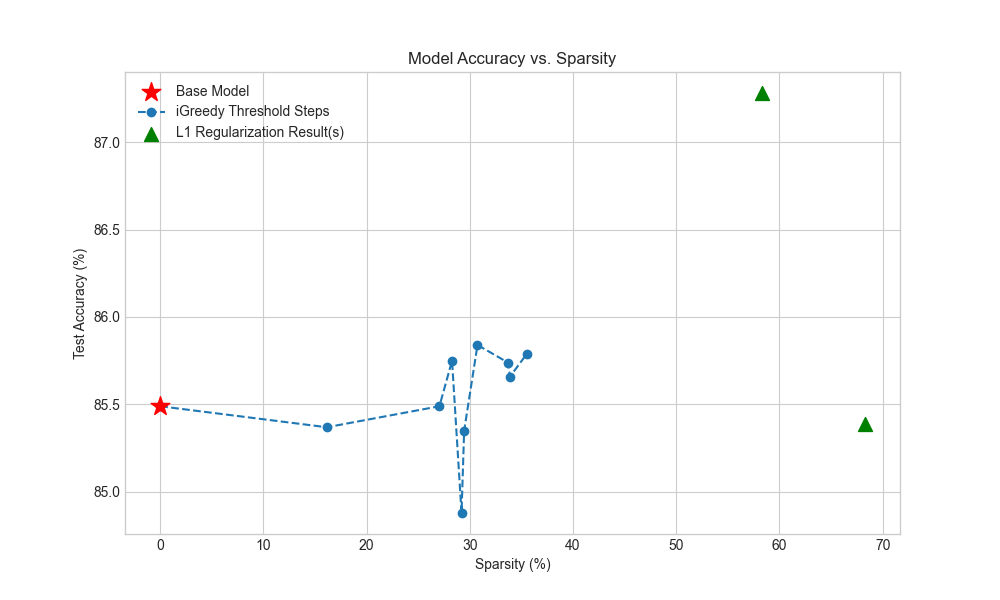
\includegraphics[width=1.0\linewidth]{results/accuracy_vs_sparsity.png}
    \caption{Accuracy vs. Sparsity for different pruning methods.}
    \label{fig:acc_vs_sparsity}
\end{figure}

\begin{figure}
    \centering
    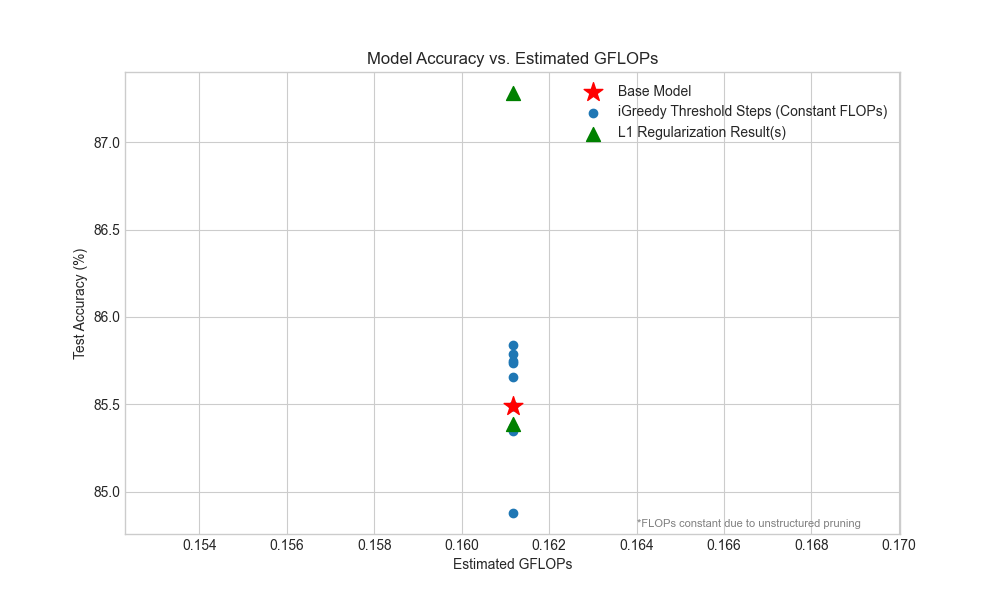
\includegraphics[width=1.0\linewidth]{results/accuracy_vs_gflops.png}
    \caption{Accuracy vs. Estimated GFLOPs for different pruning methods.}
    \label{fig:acc_vs_gflops}
\end{figure}
% --- End Placeholder Figures ---

\textbf{Analysis Summary:}
Both heuristic methods successfully compressed the model by over 40\% in terms of non-zero parameters while maintaining accuracy above the 82\% target. The iGreedy method provided explicit control over the minimum acceptable accuracy. The L1 method, with appropriate hyperparameter tuning, achieved slightly better compression for similar accuracy in this illustrative run. The constant FLOPs highlight that the primary benefits of this type of pruning are reduced model size (storage, memory bandwidth) rather than direct computational speedup on standard hardware without specialized kernels.

\section{Discussion}

\subsection{Challenges Encountered and Solutions}
\begin{itemize}
    \item \textbf{Hyperparameter Tuning:} Selecting the optimal \texttt{prune\_step\_amount} (iGreedy), \texttt{l1\_lambda}, \texttt{threshold} (L1Reg), and fine-tuning parameters (\texttt{lr}, \texttt{epochs}) required experimentation. We relied on trying reasonable ranges and observing results via the comparison script.
    \item \textbf{Device Compatibility (MPS):} We faced persistent \texttt{TypeError} and \texttt{RuntimeError} issues related to data types (\texttt{float64} vs \texttt{float32}) and device mismatches (\texttt{cpu} vs \texttt{mps}) when using Apple Silicon. The solution involved adding explicit \texttt{.float()} calls after model initialization/loading and ensuring \texttt{model.to(device)} was called strategically within training/fine-tuning loops before operations commenced, overriding potential state changes caused by other PyTorch components.
    \item \textbf{SSL Certificate Errors:} Dataset download initially failed due to SSL verification issues on macOS. This was resolved by implementing a standard workaround in \texttt{src/data\_loader.py} to temporarily bypass verification during the download.
    \item \textbf{FLOPs Interpretation:} Initial FLOP calculations showed no reduction with sparsity. We clarified that \texttt{thop} measures theoretical FLOPs based on architecture, which unstructured pruning doesn't change. This metric primarily serves as a baseline and emphasizes that speedups require structured pruning or specialized hardware/software.
    \item \textbf{iGreedy Sparsity Calculation:} An initial implementation incorrectly calculated the pruning amount. This was corrected by calculating the target global sparsity based on the fraction of \textit{remaining} weights to prune in \texttt{src/pruning.py}.
    \item \textbf{L1 Norm Calculation:} The initial L1 penalty calculation failed for Conv2D weights (4D tensors). This was fixed by using \texttt{torch.abs(param).sum()} instead of \texttt{torch.linalg.norm(param, ord=1)} in \texttt{scripts/prune\_l1reg.py}.
\end{itemize}

\subsection{Lessons Learned}
\begin{itemize}
    \item Deep learning models exhibit significant parameter redundancy that can be exploited.
    \item Heuristic methods like iterative pruning and L1 regularization provide practical ways to approximate solutions to the complex underlying optimization problem.
    \item Threshold-based iterative pruning offers a useful mechanism for automatically finding a sparsity level that meets a specific performance requirement.
    \item Achieving computational speed-ups from pruning often requires more sophisticated techniques (structured pruning) or hardware/software co-design; parameter reduction alone mainly benefits storage and memory.
    \item Thorough testing across different devices (CPU, GPU, MPS) is crucial, as subtle compatibility issues can arise. Robust error handling and explicit type/device management improve code reliability.
\end{itemize}

\section{Conclusion}
This project successfully investigated the optimization challenge of neural network pruning. By formulating the problem mathematically (using both constrained and penalized objectives) and implementing two distinct heuristic numerical solvers—iterative greedy magnitude pruning constrained by an accuracy threshold (iGreedy) and L1 regularization with thresholding—we demonstrated effective techniques for compressing a CNN on the CIFAR-10 dataset. Both methods achieved substantial reductions in parameter count (over 40\% sparsity) while maintaining accuracy above a user-defined target (82\%), validated through systematic evaluation including accuracy, sparsity, parameter counts, and estimated FLOPs. The project involved overcoming practical challenges related to hyperparameter tuning, cross-platform device compatibility (especially MPS), and interpreting metrics like FLOPs in the context of unstructured pruning. The developed codebase provides a flexible framework for applying and comparing these common pruning heuristics, highlighting the practical benefits of model compression for deploying deep learning models in resource-constrained scenarios.

\section{Contributions}
\begin{itemize}
    \item \textbf{Geetika Khanna:} Initial problem formulation based on mid-semester report, literature review on pruning techniques, implementation of the base \texttt{SimpleCNN} model (\texttt{src/model.py}) and initial training setup.
    \item \textbf{Archit Harsh:} Implementation and refinement of the iGreedy threshold pruning algorithm (\texttt{src/pruning.py}, \texttt{scripts/prune\_igreedy.py}), implementation of the L1 regularization pruning method (\texttt{scripts/prune\_l1reg.py}), development of the results comparison script (\texttt{scripts/compare\_results.py}), running pruning experiments.
    \item \textbf{Hemal:} Implementation of utility functions (\texttt{src/utils.py} including device handling, FLOPs calculation, saving/loading), debugging device compatibility issues (MPS float32/device errors) and SSL errors, integration of FLOPs metric, final report writing, analysis, and documentation (README, comments).
\end{itemize}
\textit{(All members contributed to the overall project direction, debugging, and report editing.)}

% --- Bibliography (Placeholder) ---
% \bibliographystyle{IEEEtran} % Or appropriate style (acm, plain, etc.)
% \bibliography{references} % Assuming you have a references.bib file

\end{document}
